\chapter{Peak assignments for some samples}
\label{chpt:assignments}

\epigraph{\singlespacing%
`It is over! it is over!' she repeated to herself again, and again, in nervous gratitude. `The worst is over!'
}{--- \textsc{Jane Austen}, \textit{Persuasion}}

In this appendix, I provide assignments of \proton{} and \carbon{} chemical shifts for some of the more frequently-used samples in this thesis, occasionally with some additional data.
I have made no attempt to distinguish the shifts of diastereotopic protons or methyl groups.

\clearpage 

\section{Andrographolide}

\begin{figure}[!ht]
    \centering
    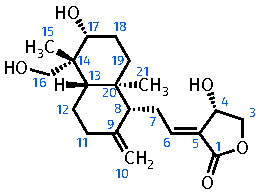
\includegraphics[draft=false,scale=1.5]{samples/andrographolide.pdf}%
    \caption[Structure of andrographolide]{
        Structure of andrographolide.
    }
    \label{fig:samples_andrographolide}
\end{figure}

\begin{table}[!ht] \begin{tabular}{ccSS}
        \toprule
        \textbf{Label in \cref{fig:samples_andrographolide}} & \textbf{Label in Claridge (2016)} & {$\symbf{\delta}$\textbf{(\proton{}) (ppm)}} & {$\symbf{\delta}$\textbf{(\carbon{}) (ppm)}} \\
        \midrule
        1     &      &              & 170.42 \\
        3     & g, i & {4.40, 4.04} & 74.80  \\
        4     & d    & 4.92         & 64.99  \\
        4-OH  & b    & 5.71         &        \\
        5     &      &              & 129.46 \\
        6     & a    & 6.63         & 146.76 \\
        7     & m, n & {2.52, 2.47} & 24.43* \\
        8     & q    & 1.87         & 55.96  \\
        9     &      &              & 148.07 \\
        10    & e, f & {4.82, 4.63} & 108.71 \\
        11    & o, p & {2.33, 1.94} & 37.98  \\
        12    & r, v & {1.75, 1.36} & 24.42* \\
        13    & w    & 1.21         & 54.84  \\
        14    &      &              & 42.75  \\
        15    & y    & 1.09         & 23.54  \\
        16    & j, k & {3.85, 3.27} & 63.11  \\
        16-OH & h    & 4.13         &        \\
        17    & l    & 3.24         & 78.91  \\
        17-OH & c    & 5.05         &        \\
        18    & t, u & {1.65, 1.65} & 28.36  \\
        19    & s, x & {1.70, 1.21} & 36.99  \\
        20    &      &              & 39.06  \\
        21    & z    & 0.67         & 15.22  \\
        \bottomrule
    \end{tabular}
    \caption[Peak assignments for andrographolide]{
        Peak assignments for andrographolide; these can also be found in Figure 9.26 (page 340) of: \fullcite{Claridge2016}.
        Asterisks indicate \carbon{} chemical shifts which could not be disambiguated.
    }
    \label{tbl:andrographolide_assignments}
\end{table}

\clearpage

\section{Cyclosporin}

\begin{figure}[!ht]
    \centering
    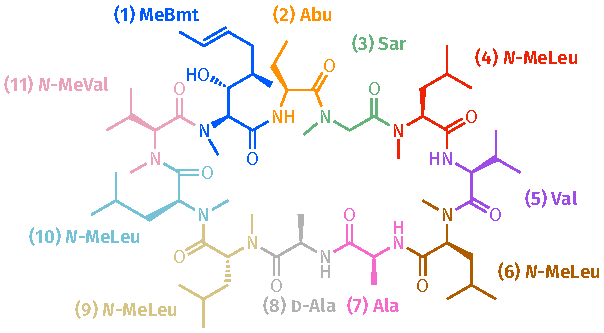
\includegraphics[draft=false,scale=1.5]{samples/cyclosporin.pdf}%
    \caption[Structure of cyclosporin]{
        Structure of cyclosporin.
    }
    \label{fig:samples_cyclosporin}
\end{figure}

\begin{spacing}{1.0}   % (tbl:cyclosporin_assignments) {{{1
\begin{longtable}{ccSSS}
    \caption[]{(continued)} \\
    \toprule
    \textbf{Residue} & \textbf{Group} & {$\symbf{\delta}$\textbf{(\proton{}) (ppm)}} & {$\symbf{\delta}$\textbf{(\carbon{}) (ppm)}} & {$\symbf{\delta}$\textbf{(\nitrogen{}) (ppm)}} \\
    \midrule
    \endhead

    \toprule
    \textbf{Residue} & \textbf{Group} & {$\symbf{\delta}$\textbf{(\proton{}) (ppm)}} & {$\symbf{\delta}$\textbf{(\carbon{}) (ppm)}} & {$\symbf{\delta}$\textbf{(\nitrogen{}) (ppm)}} \\
    \midrule
    \endfirsthead

    \caption[]{Peak assignments for cyclosporin.}
    \endfoot

    \caption[Peak assignments for cyclosporin]{
        Peak assignments for cyclosporin.
    } \label{tbl:cyclosporin_assignments}
    \endlastfoot

    1 MeBmt            & \ch{NCH3}           & 3.70         & 33.5  & 117.7 \\*
                       & $\upalpha$-\ch{CH}  & 5.69         & 59.0  &       \\*
                       & $\upbeta$-\ch{CH}   & 4.19         & 74.1  &       \\*
                       & \ch{CO}             &              & 169.9 &       \\
    \midrule
    2 Abu              & \ch{NH}             & 8.24         &       & 120.9 \\*
                       & $\upalpha$-\ch{CH}  & 5.10         & 48.7  &       \\*
                       & $\upbeta$-\ch{CH2}  & 1.76         & 25.3  &       \\*
                       & \ch{CO}             &              & 173.2 &       \\
    \midrule
    3 Sar              & \ch{NCH3}           & 3.07         & 38.6  & 112.2 \\*
                       & $\upalpha$-\ch{CH2} & 4.01         & 49.2  &       \\*
                       & \ch{CO}             &              & 170.9 &       \\
    \midrule
    4 \textit{N}-MeLeu & \ch{NCH3}           & 2.58         & 30.4  & 113.3 \\*
                       & $\upalpha$-\ch{CH}  & 5.57         & 55.3  &       \\*
                       & $\upbeta$-\ch{CH2}  & 1.35         & 36.1  &       \\*
                       & \ch{CO}             &              & 169.4 &       \\
    \midrule
    5 Val              & \ch{NH}             & 7.45         &       & 115.7 \\*
                       & $\upalpha$-\ch{CH}  & 4.87         & 55.2  &       \\*
                       & $\upbeta$-\ch{CH}   & 2.60         & 31.3  &       \\*
                       & \ch{CO}             &              & 173.8 &       \\
    \midrule
    6 \textit{N}-MeLeu & \ch{NCH3}           & 3.21         & 31.2  & 119.7 \\*
                       & $\upalpha$-\ch{CH}  & 5.37         & 55.1  &       \\*
                       & $\upbeta$-\ch{CH2}  & {2.25, 1.44} & 37.4  &       \\*
                       & \ch{CO}             &              & 171.4 &       \\
    \midrule
    7 Ala              & \ch{NH}             & 8.00         &       & 128.0 \\*
                       & $\upalpha$-\ch{CH}  & 4.78         & 48.7  &       \\*
                       & $\upbeta$-\ch{CH3}  & 1.65         & 15.8  &       \\*
                       & \ch{CO}             &              & 171.0 &       \\
    \midrule
    8 \textsc{d}-Ala   & \ch{NH}             & 7.61         &       & 119.0 \\*
                       & $\upalpha$-\ch{CH}  & 4.82         & 45.0  &       \\*
                       & $\upbeta$-\ch{CH3}  & 1.03         & 17.6  &       \\*
                       & \ch{CO}             &              & 173.9 &       \\
    \midrule
    9 \textit{N}-MeLeu & \ch{NCH3}           & 2.92         & 29.1  & 111.2 \\*
                       & $\upalpha$-\ch{CH}  & 5.85         & 48.0  &       \\*
                       & $\upbeta$-\ch{CH2}  & {2.16, 1.25} & 39.3  &       \\*
                       & \ch{CO}             &              & 170.2 &       \\
    \midrule
   10 \textit{N}-MeLeu & \ch{NCH3}           & 2.84         & 29.6  & 114.4 \\*
                       & $\upalpha$-\ch{CH}  & 5.32         & 57.5  &       \\*
                       & $\upbeta$-\ch{CH2}  & {2.40, 1.28} & 41.2  &       \\*
                       & \ch{CO}             &              & 170.1 &       \\
    \midrule
   11 \textit{N}-MeVal & \ch{NCH3}           & 2.96         & 30.1  & 117.7 \\*
                       & $\upalpha$-\ch{CH}  & 5.25         & 58.0  &       \\*
                       & $\upbeta$-\ch{CH}   & 2.25         & 29.1  &       \\*
                       & \ch{CO}             &              & 173.8 &       \\
    \bottomrule
\end{longtable}
\end{spacing}   % }}}1

\clearpage

\section{Ferulic acid}

\begin{figure}[!ht]
    \centering
    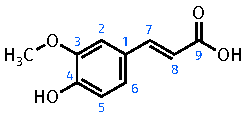
\includegraphics[draft=false,scale=1.5]{samples/ferulic.pdf}%
    \caption[Structure of ferulic acid]{
        Structure of ferulic acid.
    }
    \label{fig:samples_ferulic}
\end{figure}

\begin{table}[!ht] \begin{tabular}{cSSSS}
        \toprule
        \textbf{Label} & {$\symbf{\delta}$\textbf{(\proton{}) (ppm)}} & {$\symbf{\delta}$\textbf{(\carbon{}) (ppm)}} & {${}^{\symbf{1}}\!\symbfit{J}_{\textbf{\ch{CH}}}$ \textbf{(Hz)}} & {$\symbfit{T}_{\symbf{1}}$\textbf{(\proton{}) at \qty{600}{MHz} (s)}} \\
        \midrule
        1           &      & 126.25 &       &      \\
        2           & 7.28 & 111.62 & 157.6 & 1.15 \\
        3           &      & 148.38 &       &      \\
        3-\ch{OCH3} & 3.82 & 56.16  & 147.8 & 1.08 \\
        4           &      & 149.54 &       &      \\
        5           & 6.79 & 115.98 & 159.5 & 1.59 \\
        6           & 7.08 & 123.27 & 158.6 & 2.00 \\
        7           & 7.49 & 144.97 & 154.3 & 1.96 \\
        8           & 6.36 & 116.08 & 160.6 & 1.75 \\
        9           &      & 168.45 &       &      \\
        \bottomrule
    \end{tabular}
    \caption[Peak assignments for ferulic acid]{
        Peak assignments and other physical data for ferulic acid.
    }
    \label{tbl:ferulic_assignments}
\end{table}

\clearpage

\section{Gramicidin}

\begin{figure}[!ht]
    \centering
    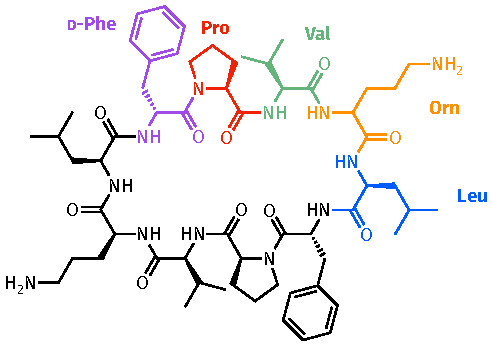
\includegraphics[draft=false,scale=1.5]{samples/gramicidin.pdf}%
    \caption[Structure of gramicidin]{
        Structure of gramicidin.
    }
    \label{fig:samples_gramicidin}
\end{figure}

\begin{table}[!ht]
    \begin{tabular}{ccSSS}
        \toprule
        \textbf{Residue} & \textbf{Group} & {$\symbf{\delta}$\textbf{(\proton{}) (ppm)}} & {$\symbf{\delta}$\textbf{(\carbon{}) (ppm)}} & {$\symbf{\delta}$\textbf{(\nitrogen{}) (ppm)}} \\
        \midrule
        Leu            & \ch{NH}                  & 8.33         &                & 123.3 \\
                       & $\upalpha$-\ch{CH}       & 4.57         & 50.09          &       \\
                       & $\upbeta$-\ch{CH2}       & {1.35, 1.29} & 41.38          &       \\
                       & $\upgamma$-\ch{CH}       & 1.41         & 24.45          &       \\
                       & $\updelta$-\ch{CH3}      & 1.41         & {23.20, 23.02} &       \\
        \midrule
        Orn            & \ch{NH}                  & 8.66         &                & 125.4 \\
                       & $\upalpha$-\ch{CH}       & 4.76         & 51.43          &       \\
                       & $\upbeta$-\ch{CH2}       & {1.75, 1.60} & 30.12          &       \\
                       & $\upgamma$-\ch{CH2}      & 1.65         & 23.52          &       \\
                       & $\updelta$-\ch{CH2}      & {2.84, 2.78} & 39.02          &       \\
                       & $\upvarepsilon$-\ch{NH2} & 8.04         &                & 36.0  \\
        \midrule
        Val            & \ch{NH}                  & 7.22         &                & 113.2 \\
                       & $\upalpha$-\ch{CH}       & 4.41         & 57.31          &       \\
                       & $\upbeta$-\ch{CH}        & 2.07         & 31.49          &       \\
                       & $\upgamma$-\ch{CH3}      & {0.80, 0.77} & {19.44, 18.50} &       \\
        \midrule
        Pro            & $\upalpha$-\ch{CH}       & 4.31         & 60.36          &       \\
                       & $\upbeta$-\ch{CH2}       & {1.95, 1.48} & 29.50          &       \\
                       & $\upgamma$-\ch{CH2}      & 1.52         & 23.58          &       \\
                       & $\updelta$-\ch{CH2}      & {3.59, 2.50} & 46.48          &       \\
        \midrule
        \textsc{d}-Phe & \ch{NH}                  & 9.09         &                & 128.0 \\
                       & $\upalpha$-\ch{CH}       & 4.36         & 54.38          &       \\
                       & $\upbeta$-\ch{CH2}       & {3.59, 2.50} & 46.48          &       \\
                       & ipso-\ch{C}              &              & 136.77         &       \\
                       & ortho-\ch{CH}            & 7.26         & 129.80         &       \\
                       & meta-\ch{CH}             & 7.29         & 128.71         &       \\
                       & para-\ch{CH}             & 7.25         & 127.34         &       \\
        \bottomrule
    \end{tabular}
    \caption[Peak assignments for gramicidin]{
        Peak assignments for gramicidin.
    }
    \label{tbl:gramicidin_assignments}
\end{table}

\clearpage

\section{Brucine}

\begin{figure}[!ht]
    \centering
    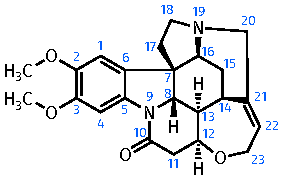
\includegraphics[draft=false,scale=1.5]{samples/brucine.pdf}%
    \caption[Structure of brucine]{
        Structure of brucine.
    }
    \label{fig:samples_brucine}
\end{figure}

\begin{table}[!ht]
    \begin{tabular}{cSSS}
        \toprule
        Label & {$\symbf{\delta}$\textbf{(\proton{}) (ppm)}} & {$\symbf{\delta}$\textbf{(\carbon{}) (ppm)}} & {$\symbf{\delta}$\textbf{(\nitrogen{}) (ppm)}} \\
        \midrule
        1           & 6.69         & 105.52 &        \\
        2           &              & 146.24 &        \\
        2-\ch{OCH3} & 3.87         & 56.46  &        \\
        3           &              & 149.25 &        \\
        3-\ch{OCH3} & 3.92         & 56.21  &        \\
        4           & 7.83         & 101.00 &        \\
        5           &              & 135.98 &        \\
        6           &              & 123.33 &        \\
        7           &              & 51.94  &        \\
        8           & 3.85         & 60.35  &        \\
        9           &              &        & 152.38 \\
        10          &              & 168.94 &        \\
        11          & {3.12, 2.67} & 42.39  &        \\
        12          & 4.30         & 77.79  &        \\
        13          & 1.28         & 48.26  &        \\
        14          & 3.16         & 31.55  &        \\
        15          & {2.37, 1.49} & 26.79  &        \\
        16          & 3.90         & 60.00  &        \\
        17          & 1.89         & 42.41  &        \\
        18          & {3.22, 2.87} & 50.21  &        \\
        19          &              &        & 40.55  \\
        20          & {3.73, 2.75} & 52.71  &        \\
        21          &              & 140.32 &        \\
        22          & 5.92         & 127.54 &        \\
        23          & {4.16, 4.07} & 64.60  &        \\
        \bottomrule
    \end{tabular}
    \caption[Peak assignments for brucine]{
        Peak assignments for brucine.
    }
    \label{tbl:brucine_assignments}
\end{table}

\clearpage

\section{Zolmitriptan}

\begin{figure}[!ht]
    \centering
    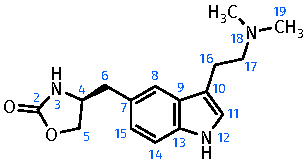
\includegraphics[draft=false,scale=1.5]{samples/zolmitriptan.pdf}%
    \caption[Structure of zolmitriptan]{
        Structure of zolmitriptan.
    }
    \label{fig:samples_zolmitriptan}
\end{figure}

\begin{table}[!ht]
    \begin{tabular}{cSSSS}
        \toprule
        Label & {$\symbf{\delta}$\textbf{(\proton{}) (ppm)}} & {$\symbf{\delta}$\textbf{(\carbon{}) (ppm)}} & {$\symbf{\delta}$\textbf{(\nitrogen{}) (ppm)}} & {${}^{\symbf{1}}\!\symbfit{J}_{\textbf{\ch{CH}}}$ \textbf{(Hz)}} \\
        \midrule
        2  &              & 159.16 &       &                \\
        3  & 7.77         &        & 89.2  &                \\
        4  & 4.05         & 53.64  &       & 146.7          \\
        5  & {4.23, 4.03} & 68.54  &       & {153.0, 151.7} \\
        6  & {2.90, 2.79} & 41.11  &       & {127.7, 127.1} \\
        7  &              & 126.32 &       &                \\
        8  & 7.37         & 119.24 &       & 155.4          \\
        9  &              & 127.99 &       &                \\
        10 &              & 112.92 &       &                \\
        11 & 7.12         & 123.18 &       & 179.7          \\
        12 & 10.71        &        & 129.6 &                \\
        13 &              & 135.64 &       &                \\
        14 & 7.26         & 111.71 &       & 158.9          \\
        15 & 6.93         & 122.97 &       & 155.7          \\
        16 & 2.81         & 23.55  &       & 125.8          \\
        17 & 2.53         & 60.46  &       & 132.2          \\
        18 &              &        & 106.6 &                \\
        19 & 2.26         & 45.65  &       & 132.5          \\
        \bottomrule
    \end{tabular}
    \caption[Peak assignments for zolmitriptan]{
        Peak assignments and other physical data for zolmitriptan.
    }
    \label{tbl:zolmitriptan_assignments}
\end{table}
